\documentclass[palatino,nobuilddate,nochap]{apuntesURJC}

\title{Práctica de Modelización}
\subtitle{Matemáticas para la vida cotidiana}
\author{Víctor de Juan, Gustavo Martínez y Virginia Vadillo}
\date{16/17 C2}

% Paquetes adicionales

% --------------------

\newcommand{\espaciover}[0]{0.7cm}

\begin{document}

\maketitle
% Contenido.


\section{Para profesores}

\subsection{Delimitación del Contexto y forma de trabajo}
Esta práctica está destinada a alumnos de Matemáticas Aplicadas a las Ciencias Sociales I que se imparte en 1º de Bachillerato.

\subsection{Objetivos}

Los objetivos que se pretenden conseguir con esta practica son:
\begin{enumerate}
	\item Afianzar el concepto de cociente incremental.
	\item Obtener la fórmula de la ecuación de la recta tangente a una gráfica en un punto.
	\item Aplicar matemáticas de curso anteriores (la ecuación punto-pendiente, temario de 4 ESO) y darle continuidad al currículo.
	\item Orientar al alumno para que sea él quien llegue a los resultados razonando y no memorizando o repitiendo razonamientos del profesor.
\end{enumerate}

\paragraph{Objetivos secundarios}
\begin{itemize}
	\item Obtener la fórmula de la ecuación de la recta normal a una gráfica en un punto.
	\item Reforzar y repasar la geometría de 4 ESO (ecuación de la recta punto-pendiente).
\end{itemize}


\subsection{Conocimientos previos necesarios}
\begin{enumerate}
	\item Derivabilidad. Qué es la derivada de una función. Calcular derivadas sencillas.
	\item Representación gráfica de rectas. Obtención de pendientes.
\end{enumerate}

\subsection{Temas que se trabajarán}
Los temas que se van a trabajar en esta práctica son los siguientes: 
\begin{enumerate}
	\item Ecuación punto-pendiente.
	\item Obtención de pendientes.
	\item Representación gráfica de rectas. 
	\item Cálculo de derivadas sencillas. 
	\item Límites.
\end{enumerate}

\subsection{Organización de la práctica}
La práctica será realizada de manera individual por cada alumno.

\subsection{Recursos necesarios}
El profesor, aparte del guión de la práctica proporcionará las clásicas hojas de papel milimetrado con el que los alumnos puedan dibujar las rectas con mayor precisión.
\newpage

\section{Desarrollo y guión para el alumnado}

\subsection{Presentación del problema}
La experiencia de años como docentes nos ha permitido conocer los problemas habituales que suelen tener los alumnos de 1ª de Bachillerato a la hora de entender el concepto de recta pendiente a una curva en un determinado punto de la curva. Este concepto es fundamental en las matemáticas de 1º de Bachillerato y entender en detalle cual es su significado será de gran ayuda para el desarrollo de este curso y posteriores.

\newpage
\subsection{Bloque I: Ecuación de la recta dada un punto y una pendiente}

\subsubsection{Concepto y cálculo de la pendiente de una recta}
\begin{enumerate}
	\item Por cada una de las rectas que ves en las imágenes, determina por cada cuadro que se desplaza la recta hacia a la derecha en el eje horizontal, ¿cuántos cuadros se desplaza en la vertical?
	
	\begin{table}[hbtp]
		\centering
		\begin{tabular}{|c|c|c|c|}
			\hline
			a)&b)&c)&d)\\\hline
			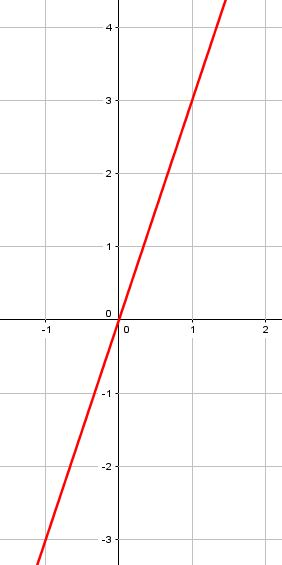
\includegraphics[scale=0.3]{img/EjemploPendiente01.JPG}& 
			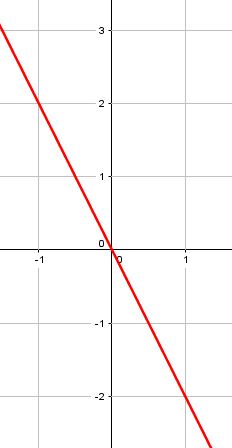
\includegraphics[scale=0.4]{img/EjemploPendiente02.JPG}& 
			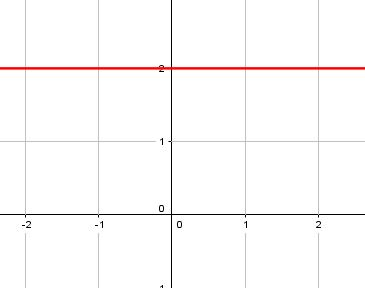
\includegraphics[scale=0.5]{img/EjemploPendiente03.JPG}& 
			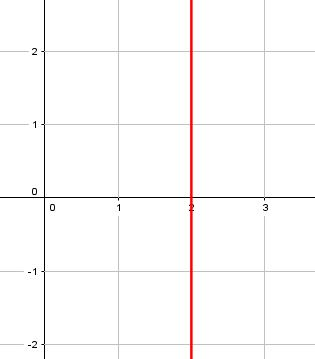
\includegraphics[scale=0.4]{img/EjemploPendiente04.JPG}
			\\\hline			
		\end{tabular}
		\caption{}
		\label{tbl_ejemplosPendiente}
	\end{table}
	
	\item ¿Qué es la pendiente de una recta? ¿Cómo se puede medir? ¿Ves alguna relación con el apartado anterior?
	\vspace{\espaciover}

	\item Calcular la pendiente de las rectas de la figura \ref{RectasParaPendientes}:

	\begin{figure}[h]
		\centering
		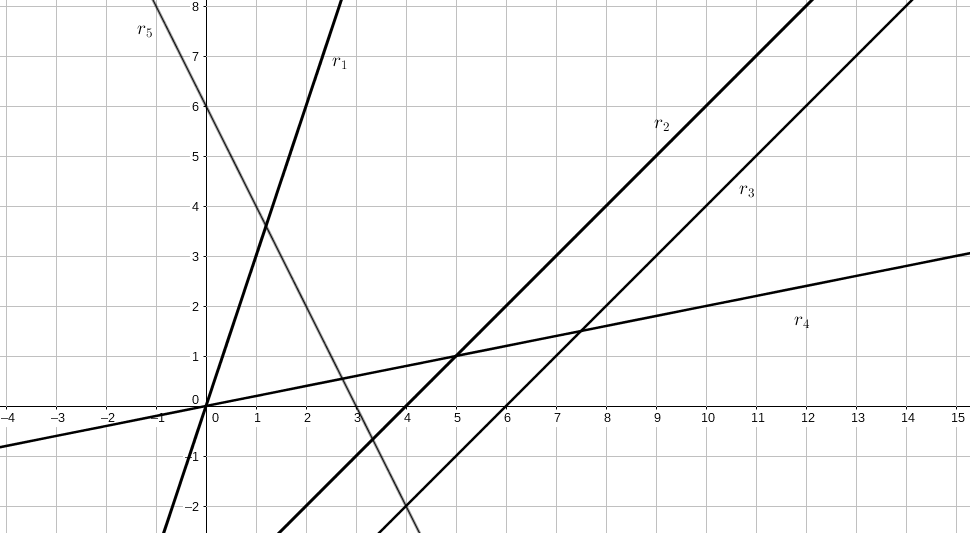
\includegraphics[scale=0.4]{img/rectas.png}
		\caption{Rectas para calcular sus pendientes}
		\label{RectasParaPendientes}
	\end{figure}

	\vspace{\espaciover}

	\item Paralelismo:
	\subitem Dadas 2 rectas paralelas, ¿cómo son sus pendientes?
	\vspace{\espaciover}

	\subitem Dadas 2 rectas con la misma pendiente, ¿se cortan en algún punto?
	\vspace{\espaciover}

	\item ¿Qué pendiente tiene una recta horizontal? \footnote{Pista: las rectas 
	horizontales son de la forma $y=a$.}
	\vspace{\espaciover}

	%\item \textit{Tiene truco} ¿Qué pendiente tiene una recta vertical? \footnote{Pista: las rectas verticales son de la forma $x=b$.}	\vspace{\espaciover}
\end{enumerate}


\subsubsection{Rectas que pasan por puntos y puntos que pertenece a rectas}
Completa la tabla \ref{tbl_puntospertenecen}, indicando si el punto (indicado por la fila) pertenece a la recta (indicado por la columna).

\begin{table}[hbtp]
\centering
\begin{tabular}{|c||c|c|c|c|}
\hline
\textbf{Recta:} & $y=3x$ & $y = 3x-9 = 3·(x-3)$ & $y - 6 = 3x$ & $y - 6 = 3x - 9$\\\hline
(0,0) &&&&\\\hline
(0,3) &&&&\\\hline
(3,0) &&&&\\\hline
(6,0) &&&&\\\hline
(0,6) &&&&\\\hline
(6,3) &&&&\\\hline
(3,6) &&&&\\\hline
\end{tabular}
\caption{}
\label{tbl_puntospertenecen}
\end{table}

\subsubsection{Construir rectas dados un punto y una pendiente}

Insipirándote en la tabla \ref{tbl_puntospertenecen}, intenta contestar a las siguientes preguntas.

\begin{enumerate}
	\item La tabla \ref{tbl_puntospertenecen} es solamente un ejemplo. ¿Podemos escribirlo de una manera más general? Es decir, si la recta $y=m·x$, siendo $m$ la pendiente, ¿qué podemos escribir para asegurar que la recta pasa por el punto $(x_0,y_0)$?
	
	\vspace{3cm}
	
	\item Utilizando la expresión del apartado anterior, escribe la ecuación de la recta con los datos de la tabla \ref{tbl_ecuaciones}

	\begin{table}[hbtp]
	\centering
	\begin{tabular}{|c|c||c|}
	\hline
	Punto & Pendiente & Ecuación de la recta\\\hline
	(0,0) & 2 & \\\hline
	(2,3) & 2 & \\\hline
	(6,2) & 1 & \\\hline
	(0,-3) & -5 & \\\hline
	\end{tabular}

	\caption{}
	\label{tbl_ecuaciones}
	\end{table}

\end{enumerate}

\newpage
\subsection{Bloque II: Cociente incremental}

\paragraph{Recta que pasa por 2 puntos dada una gráfica}

\subparagraph{Puntos en la gráfica}
Observa la gráfica de $f(x)=x^2-3$
\begin{figure}[h]
\centering
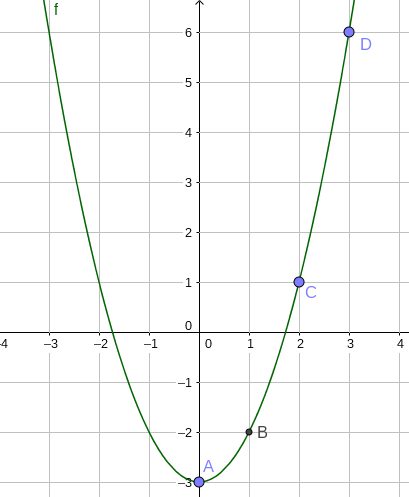
\includegraphics[scale=0.5]{img/parab.png}
\caption{Gráfica de la función $f(x) = x^2-3$}
\label{GraficaXcuad}
\end{figure}

\begin{enumerate}
	\item ¿Qué coordenada vertical tiene el punto de coordenada horizontal $x=1.5$ si sabemos que pertenezca a la gráfica? (\textit{Sol: -0.75})
	\item ¿Qué distancia \textit{horizontal} separa $A$ de $B$? ¿Y de $C$? ¿Y de $D$?
	\item Escribe las coordenadas de $B,C,D$ en función de las de $A$.
	\item Escribe las coordenadas de un punto genérico de la función a una distancia \textit{horizontal} $h$ del punto $A$. 
\end{enumerate}


\subparagraph{Recta que pasa por 2 puntos de una gráfica}
\begin{enumerate}
	\item Calcula analíticamente la pendiente de la recta que pasa por A y por D. Compruébalo calculando la pendiente gráficamente.
	\item Calcula analíticamente la pendiente de la recta que pasa por A y por C. Compruébalo calculando la pendiente gráficamente.
	\item Calcula analíticamente la pendiente de la recta que pasa por A y por B. Compruébalo calculando la pendiente gráficamente.
	\item Si cada vez acercamos más el punto, ¿qué ocurre con la recta? Es decir, imagina un punto $A'$ todo lo cercano a $A$ que quieras. 
	%
	Entre $A$ y $A'$ existirá una distancia horizontal que podemos llamar, como antes, $h$. Calcula la pendiente de esta recta.
	\item ¿Y si hacemos tender $h$ a 0? Escribe el límite cuando $h$ tiene a 0 de la pendiente. ¿Te suena de algo este límite? ¿Tiene algún nombre especial? 
	%
	\subitem En el límite, ¿podemos seguir diciendo que la recta pasa por 2 puntos? Es decir, ¿cómo es esta recta? 
\end{enumerate}

\vfill

\subsection{Bloque III: Derivadas}

Con todos los pasos previos, calcula:

\begin{enumerate}
	\item La recta tangente a la gráfica de la función $y=3x^3$ en el punto $x=2$. Para ello:
	\subitem Calcula la pendiente que tendrá esa recta.
	\subitem Calcula la coordenada vertical del punto $x=2$.
	\subitem Escribe la ecuación de la recta.
	\vspace{2cm}
	\item La recta tangente a la gráfica de la función $y=e^x$ en el punto $x=0$.
	\item La recta tangente a la gráfica de una función cualquiera $y=f(x)$ en un punto cualquiera $x_0$.
\end{enumerate}
\vspace{3cm}
\newpage
\subsection{Bloque IV: La recta normal (extra)}

\begin{figure}[hbtp]
\centering
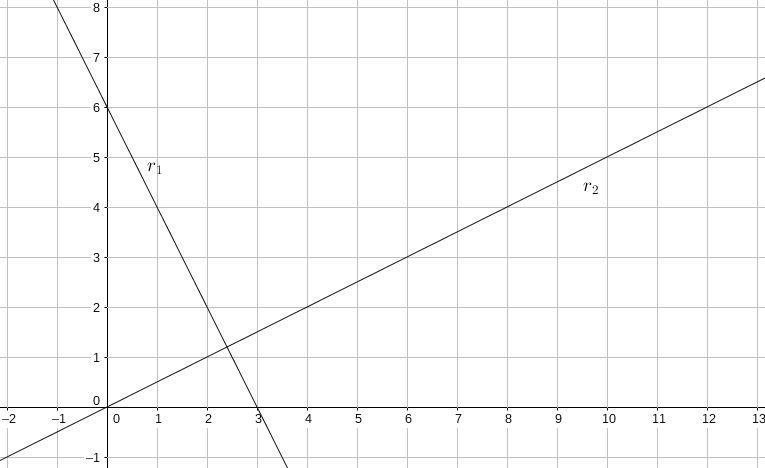
\includegraphics[scale=0.6]{img/perpen.png}
\caption{}
\label{img:perpen}
\end{figure}


Atendiendo a la figura \ref{img:perpen} contesta:
\begin{enumerate}
	\item ¿Cómo son estas rectas?
	\item ¿Cómo es el producto de las pendientes de cada recta?
	\item ¿Serían perpendiculares las rectas $y=3x$ e $y=\frac{-x}{3}-2$?
	\item \textbf{Definición:} la recta \textbf{normal} a una gráfica en un punto es la recta perpendicular a la recta tangente a la gráfica en ese mismo punto.
	\subitem ¿Sabrías calcular la ecuación de la recta normal en los 3 casos del bloque III?
\end{enumerate}

\newpage
\subsection{Evaluación}
Los criterios que se han seguido para evaluar a los alumnos son los siguientes:
\begin{enumerate}
	\item Grado de consecución de objetivos.
	\item Uso adecuado de los conocimientos previos.
	\item Autonomía.
	\item Rapidez y agilidad en las respuestas.
	\item Capacidad de análisis.
	\item Resolución del bloque de ampliación.
\end{enumerate}


%% Apendices (ejercicios, examenes)

\printindex
\end{document}
